\section{Сжатое представление леса разбора}

Матричный алгоритм даёт нам ответ на вопрос о достижимости, но не предоставляет самих путей.
Что делать, если мы хотим построить все пути, удовлетворяющие ограичениям?

Проблема в том, что искомое множество путей может быть бесконечным.
Можем ли мы предложить конечную структуру, однозначно описывающую такое множество?
Вспомним, что пересечение контекстно-свободного языка с регулярным --- это контекстно-свободный язык.
Мы знаем, что конекстно-свободный язык можно описать коньекстно-своюодной граммтикой, которая конечна.
Это и есть решение нашего вопроса. 
Осталось толко научиться строить такую грамматику.

Прежде, чем двинуться дальше, рекомендуется вспомнить всё, что касается деревьев вывода~\ref{sect:DerivTree}.

\subsection{Лес разбора как представление контекстно-свободной грамматики}

Для начала нам потребуется внести некоторые изменения в конструкцию дерева вывода.

Во-первых, заметим, что в дереве вывода каждый узел соответсвует выводу какой-то подстроки с известными позициями начала и конца.
Давайте будем сохранять эту информацию в узлах дерева. 
Таким образом, метка любого узла это тройка вида $(i,q,j)$, где $i$ --- координата начала подстроки, соответствующей этому узлу, $j$ --- координата конца, $q \in \Sigma \cup N$ --- метка как в исходном определении.

Во-вторых, заметим, что внутренний узел со своими сыновьями связаны с продукцией в граммтике: узел появляется благодаря применению конкретной продукции в процессе вывода.
Давайте занумеруем все продукции в граммтике и добавим в дерево вывода ещё один тип узлов (дополнительные узлы), в которых будем хранить номер применённой продукции.
Получим следующую конструкцию: непосредственный предок дополнительного узла --- это левая часть продукции, а непосредственные сыновья дополнительного узла --- это правая часть продукции.  

\begin{example}
  Построим модифицированное дерево вывода цепочки $_0a_1b_2a_3b_4a_5b_6$ в грамматике

  \begin{align*}
   G = \langle &&& \{a,b\}, \{S\},  S, \\
  & \{ && \\
       && (0) S & \to a \ S \ b \ S, \\
       && (1) S & \to \varepsilon \\
  & \} && \\ 
  &&& \rangle 
  \end{align*}

\begin{center}

    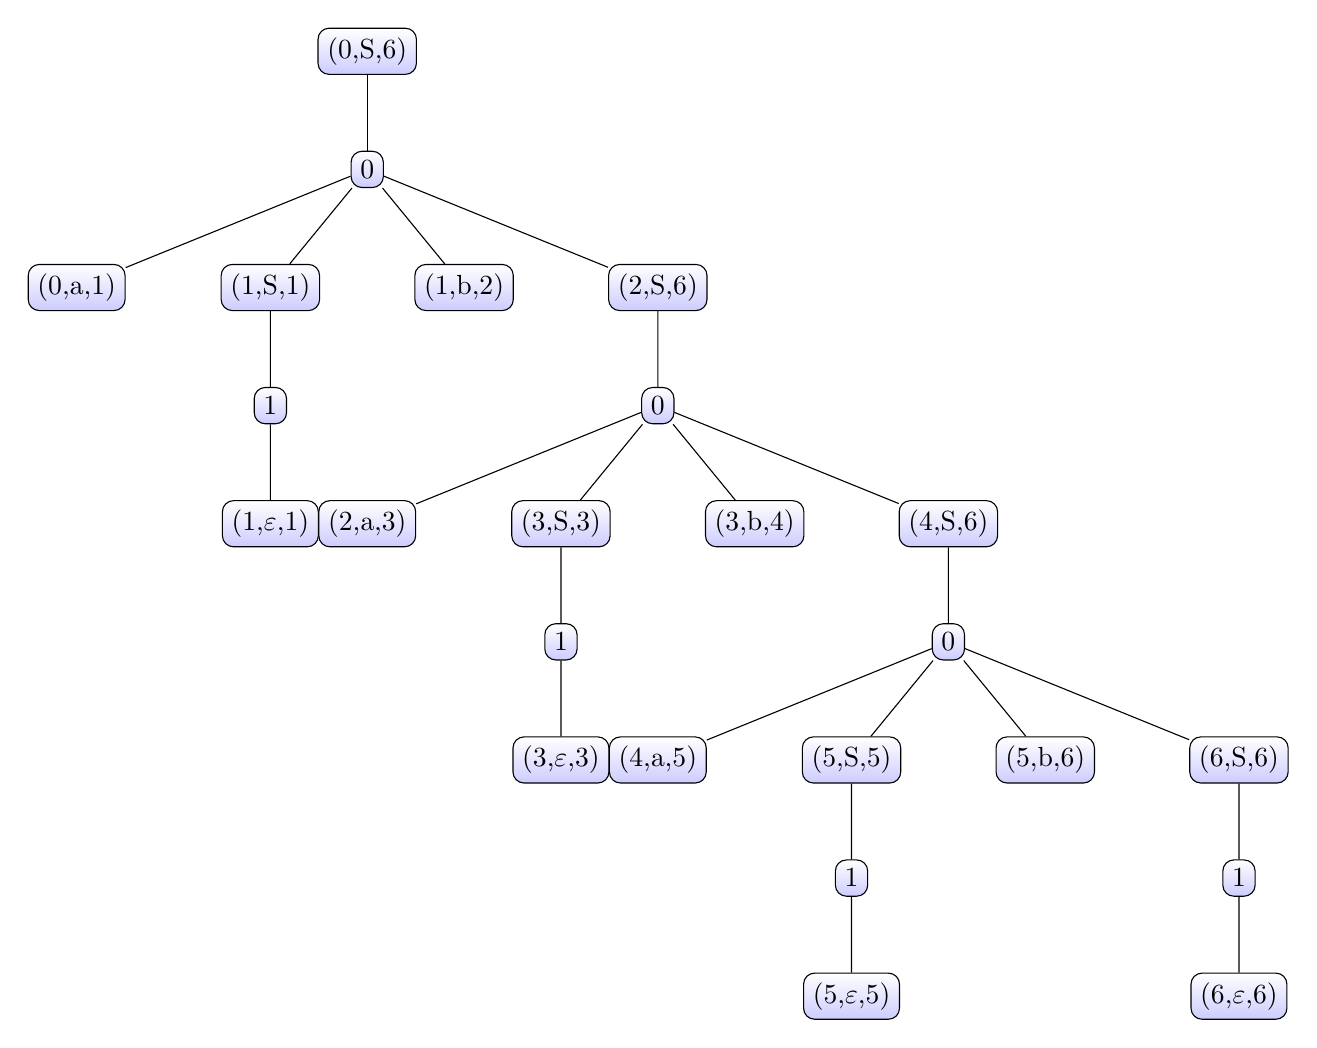
\begin{tikzpicture}[sibling distance=7em,
    every node/.style = {shape=rectangle, rounded corners,
      draw, align=center,
      top color=white, bottom color=blue!20}]]
    \node {(0,S,6)}
      child {node {0}
        child { node {(0,a,1)} }
        child { node {(1,S,1)}
          child { node {1}
            child { node {(1,$\varepsilon$,1)}}
            }
          }
      child { node {(1,b,2)} }
      child { node {(2,S,6)}
         child { node {0}
            child {node {(2,a,3)}}
            child { node {(3,S,3)}
              child { node {1}
                child { node {(3,$\varepsilon$,3)}}
              }
            }
            child { node {(3,b,4)} }
            child { node {(4,S,6)}
              child { node {0}
                child {node {(4,a,5)}}
                child {node {(5,S,5)}
                  child { node {1}
                    child {node {(5,$\varepsilon$,5)}}
                  }
                }
                child {node {(5,b,6)}}
                child {node {(6,S,6)}
                  child { node {1}
                    child {node {(6,$\varepsilon$,6)}}
                  }
                }
              }
            }
          }
        }
      };
  \end{tikzpicture}
\end{center}

\end{example}


Сохраняемая нами дополнительная информация позволит переиспользовать узлы в том случае, если деревьев вывода оказалось несколько (в случае неоднозначной грамматики).
При этом мы можем не бояться, что переиспользование узлов может привести к появлению ранее несуществовавших деревьев вывода, так как дополнительная информация позволяет делать только ``безопасные'' склейки и затем восстанавливать только корректные деревья.


\begin{example}
  Сжатие леса вывода.
  Построим несколько деревьев вывода цепочки $_0a_1b_2a_3b_4a_5b_6$ в грамматике

  \begin{align*}
   G_1 = \langle &&& \{a,b\}, \{S\},  S, \\
  & \{ && \\
       && (0) S & \to S S, \\
       && (1) S & \to a \ S \ b, \\
       && (2) S & \to \varepsilon \\
  & \} && \\ 
  &&& \rangle 
  \end{align*}

Дерево раз

\begin{center}

    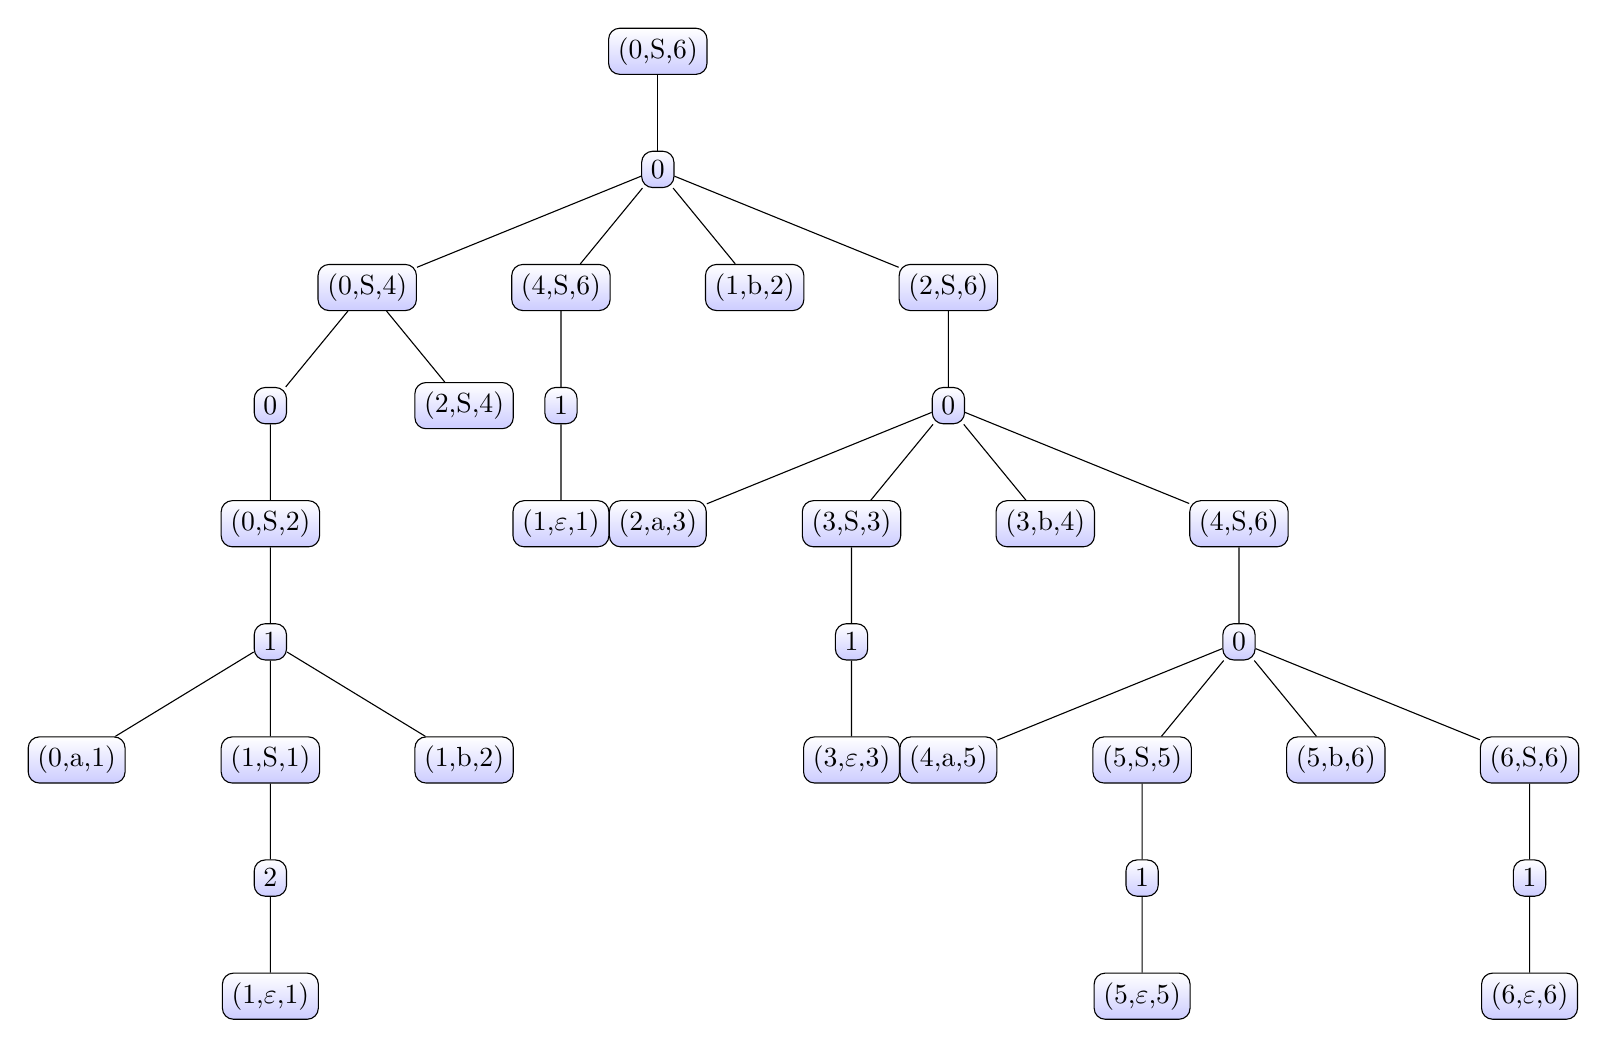
\begin{tikzpicture}[sibling distance=7em,
    every node/.style = {shape=rectangle, rounded corners,
      draw, align=center,
      top color=white, bottom color=blue!20}]]
    \node {(0,S,6)}
      child {node {0}
        child { node {(0,S,4)} 
          child {node {0}
            child { node {(0,S,2)}
              child { node {1}
                child { node {(0,a,1)} }
                child { node {(1,S,1)}
                  child { node {2}
                    child {node {(1,$\varepsilon$,1)} }
                  }
                }
                child { node {(1,b,2)} }
              }
            }
          }
          child { node {(2,S,4)}
          }
        }
        child { node {(4,S,6)}
          child { node {1}
            child { node {(1,$\varepsilon$,1)}}
            }
          }
      child { node {(1,b,2)} }
      child { node {(2,S,6)}
         child { node {0}
            child {node {(2,a,3)}}
            child { node {(3,S,3)}
              child { node {1}
                child { node {(3,$\varepsilon$,3)}}
              }
            }
            child { node {(3,b,4)} }
            child { node {(4,S,6)}
              child { node {0}
                child {node {(4,a,5)}}
                child {node {(5,S,5)}
                  child { node {1}
                    child {node {(5,$\varepsilon$,5)}}
                  }
                }
                child {node {(5,b,6)}}
                child {node {(6,S,6)}
                  child { node {1}
                    child {node {(6,$\varepsilon$,6)}}
                  }
                }
              }
            }
          }
        }
      };
  \end{tikzpicture}
\end{center}

Дерево два.

Результат сжатия.

\end{example}


Мы получили сжатое представление леса разбора (Shared Packed Parse Forest, SPPF). 
Впервые идея была предложена Джоаном Рекерсом в его кандидатской диссертации~\cite{SPPF}.
Существуют различные вариации: бинаризованное, для расширенных граммтик.

Вообще говоря, никто не мешает иметь в этом лесу циклы. 
При линейном случае тоже могут быть --- эпсилон-циклы.

А у нас будут произвольные.

Давайте пока методом пристольного взгляда.


Заметим, что это грамматика..


Ну а дальше будем смотреть на алгоритмы, которые что-то таое умеют строить.



\subsection{Вопросы и задачи}
\begin{enumerate}
  \item Постройте дерево вывода цепочки $w=aababb$ в грамматике $G=\langle\{a,b\},\{S\},\{S\rightarrow \varepsilon \ | \ a \ S \ b \ S \}, S \rangle$.
  \item Постройте все левосторонние выводы цепочки $w=ababab$ в грамматике $G=\langle\{a,b\},\{S\},\{S\rightarrow \varepsilon \ | \ a \ S \ b \ | S \ S\}, S \rangle$.
  \item Постройте все правосторонние выводы цепочки $w=ababab$ в грамматике $G=\langle\{a,b\},\{S\},\{S\rightarrow \varepsilon \ | \ a \ S \ b \ | S \ S\}, S \rangle$.
  \item \label{t1}Постройте все деревья вывода цепочки $w=ababab$ в грамматике $G=\langle\{a,b\},\{S\},\{S\rightarrow \varepsilon \ | \ a \ S \ b \ | S \ S\}, S \rangle$, соответствующие левосторонним выводам.
  \item \label{t2}Постройте все деревья вывода цепочки $w=ababab$ в грамматике $G=\langle\{a,b\},\{S\},\{S\rightarrow \varepsilon \ | \ a \ S \ b \ | S \ S\}, S \rangle$, соответствующие правосторонним выводам.
  \item Как связаны между собой леса, полученные в предыдущих двух задачах (\ref{t1} и \ref{t2})? Какие выводы можно сделать из такой связи?
  \item Постройте сжатое представление леса разбора, полученного в задаче~\ref{t1}.
  \item Постройте сжатое представление леса разбора, полученного в задаче~\ref{t2}.
  \item \label{t3}Предъявите контекстно-свободную граммтику существенно неоднозначного языка. 
        Возьмите цепочку длины болше пяти, при надлежащую этому языку, и постройте все деревья вывода этой цепочки в предъявленной граммтике. 
  \item Постройте сжатое представление леса, полученного в задаче~\ref{t3}.
\end{enumerate}
